Funkcija je relacija kod koje se svakom elementu prvog skupa pridružuje točno jedan element drugog skupa.
Funkcija nekom argumentu iz domene pravilom pridruživanja odrešuje vrijednost iz kodomene.
Postoje razne vrste funkcija poput linearne, logaritamske i drugih i razna svojstva funkcija.
Funkcije označavamo ovako:
\[f \colon D_f \to K_f\]
\[x \mapsto f(x)\]
Ovaj zapis nam govori da funkcija \(f\) preslikava vrijednost iz domene \(D_f\) u kodomenu \(K_f\) i da pravilo pridruživanja argumentu \(x\) pridružuje vrijednost \(f(x)\) tj. da se \(x\) mapira u \(f(x)\).
Češće se s funkcija susrećemo u obliku funkcijske notacije koju je prvi koristio Euler.
Funkcijska notacija sastoji se od ukošog latiničnog slova koje slijede zagrade unutar koji se nalazi argument.
\[y = f(x)\]
Graf funkcije je skup uređenih parova argumeneta i vrijednosti neke funkcije:
\[\Gamma_f = \{(x, y) \colon x \in D_f, y = f(x)\}\]
Graf funkcije najčešće crtamo u Kartezijevom koordinatnom sustavu radi lakše predodžbe funkcije.
Funkcije se najčešće koriste kako bi prikazali ovisnost jedne vrijednosti o drugoj.
Funkcijama se modeliraju prirodne pojave.

\subsection{Domena i kodomena funkcije}
    Domena ili područje definicije funkcije je skup argumenata za koje je funkcija definirana.
    Da je funkcija definirana za neki argument znači da vraća vrijednost za taj argument.
    Domena se grafički prikazuje kao x-os Kartezijevog koordinatnog sustava. 
    \\
    Prirodna domena je maksimalna domena neke funkcije, dakle najveći skup vrijednosti za koje zadani zakon pridruživanja ima smisla.
    \begin{figure}[ht]
        \centering
        \begin{tikzpicture}[
            every node/.style={on grid},
            setA/.style = {fill=black, circle, inner sep=1pt},
            setB/.style = {fill=black, circle, inner sep=1pt},
            every fit/.style = {draw, ellipse, text width=25pt},
            >=latex
        ]
            \node[setA, label=left:$a$] (a) {};
            \node[setA, below = of a, label=left:$b$] (b) {};
            \node[setA, below = of b, label=left:$c$] (c) {};
            \node[above = of a, anchor = south] {$D_f$};
          
            \node[setB, label=right:$x$, right = 3cm of a] (x) {};
            \node[setB, label=right:$y$, below = of x] (y) {};
            \node[setB, label=right:$z$, below = of y] (z) {};
            \node[above = of x, anchor = south] {$K_f$};
          
            \draw[->,shorten >= 3pt] (a) -- node[label=above:$f$] {} (x);
            \draw[->,shorten >= 3pt] (b) -- node[label=above:$f$] {} (y);
            \draw[->,shorten >= 3pt] (c) -- node[label=above:$f$] {} (z);
            
            \begin{pgfonlayer}{background}
                \node[fit = (x) (z) ] {};
                \node[fit = (a) (c) ] {};
            \end{pgfonlayer}
        \end{tikzpicture}
        \caption{Grafički prikaz preslikavanja vrijednosti \(a, b, c\) iz domene \(D_f\) u \(x, y, z\) iz kodomene \(K_f\)} 
        \label{fig:template}
    \end{figure}
    Kodomena funkcije je skup na koji su njezine funkcijske vrijdnosti ograničene.
    Slika funkcija je skup svih funkcijskih vrijdnosti funkcije tj. najmanja kodomena. Označavamo je \(Im(f)\).
    
\subsection{Nultočke i točke u kojima graf sječe y-os \label{nultočke}}
    Nultočke funkcije su točke u kojima graf funkcije sijeće x-os, odnosno uređeni parovi argumenta i vrijenosti \(0\).
    Pošto je x-os zadana funkcijom:
    \[f_x(x) = 0\]
    nultočke se nalaze na x-osi pa zadovoljavaju funkciju gore, možemo ih definirati kao sljedeći skup:
    \[\{(x, f_x(x)) \colon x \in D_f \mid f(x) = f_x(x)\} = \{(x, 0) \colon x \in D_f \mid f(x) = 0\}\]
    \clearpage
    \noindent Točka u kojoj graf sječe y-os je definirana uređenim parom gdje je argument jednak nuli.
    \[(0, f(0))\]
    Za razliku od nultočaka takva je točka samo jedna zbog toga što funkcija svakom argumentu pridružuje samo jednu vrijednost.
    \begin{figure}[ht]
        \centering
        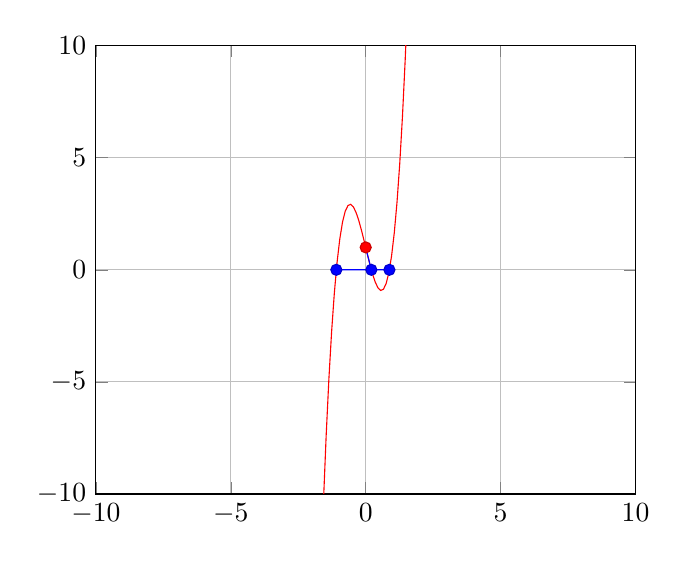
\begin{tikzpicture}
            \begin{axis}[
                grid=major,
                ymin=-10,
                ymax=10,
                xmin=-10,
                xmax=10,
            ]
                \addplot[
                    color = red,
                    samples = 100
                ]{5 * x^3 - 5 * x + 1};
                \addplot[
                    color = blue,
                    scatter
                ]coordinates{
                    (-1.088033, 0) (0.878885, 0) (0.209148, 0) (0, 1)
                };
            \end{axis}
        \end{tikzpicture}
        \caption{Graf kubne funkcije s označenim nultočkama i sjecištem u y-osi} 
        \label{fig:template}
    \end{figure}
    \\
    Osnovni teorem algebre nam veli da polinomska funkcija \(n\)-tog stupnja ima \(n\) nultočaka (valja imati na umu da te nultočke nisu nužno realne).


\subsection{Parnost i neparnost \label{par}}
    Parne i neparne funkcije su funkcije čiji su grafovi simetrične na određen način.
    Grafovi parnih funkcija su osno simetrični s obzirom na y-os pa vrijedi:
    \[f(x) = f(-x)\]
    Primjer parne funkcije je kosinus.
    \begin{figure}[ht]
        \centering
        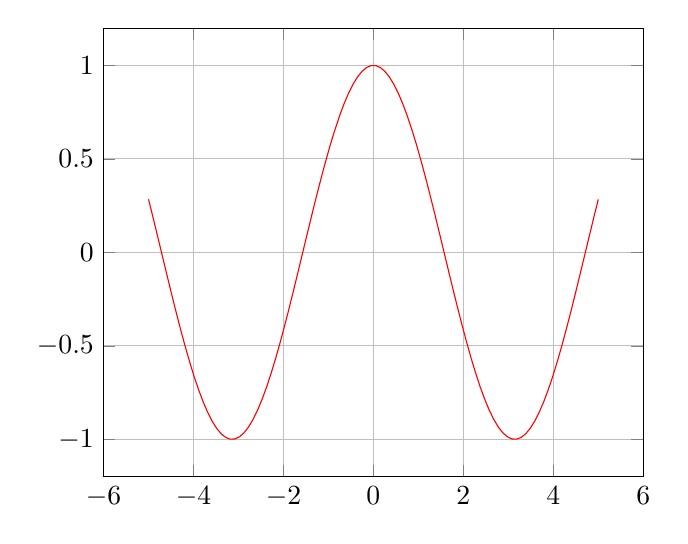
\begin{tikzpicture}
            \begin{axis}[
                grid=major,
            ]
                \addplot[
                    color = red,
                    samples = 100
                ]{cos(deg(x))};
            \end{axis}
        \end{tikzpicture}
        \caption{Graf funkcije \(f(x) = cos(x)\)} 
        \label{fig:template}
    \end{figure}
    \\
    Grafovi neparnih funkcije su centralno simentrične s obzirom na ishodište koordinatnog sustava i za njih vrijedi:
    \[-f(x) = f(-x)\]
    \clearpage
    \noindent Primjer parne funkcije je kosinus.
    \begin{figure}[ht]
        \centering
        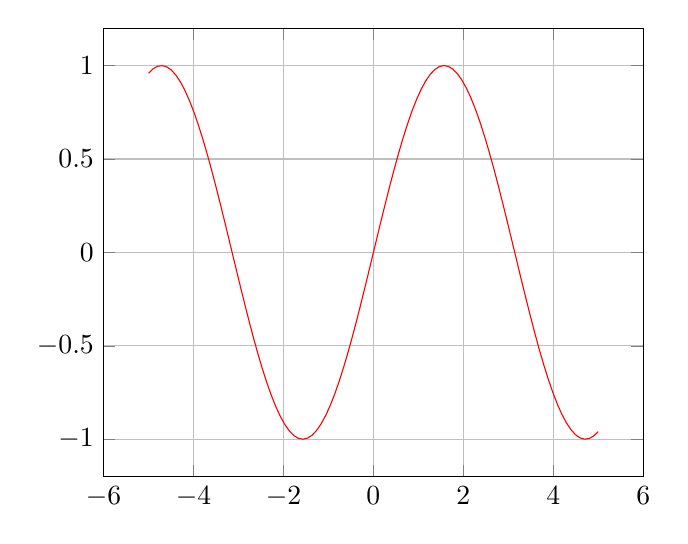
\begin{tikzpicture}
            \begin{axis}[
                grid=major,
            ]
                \addplot[
                    color = red,
                    samples = 100
                ]{sin(deg(x))};
            \end{axis}
        \end{tikzpicture}
        \caption{Graf funkcije \(f(x) = sin(x)\)} 
        \label{fig:template}
    \end{figure}
    \\
    Parnost i neparnost nisu isključiva svojstva (primjer: \(f(x) = 0\)).
    Polinomske funkcije parnog stupnja su parne, a polinomske funkcije neparnog stupnja neparne.

\subsection{Periodičnost}
    Periodnične funkcije su funkcije čije se vrijednosti ponavljaju u pravilnim razmacima.
    Funkcija je periodična ako vrijedi:
    \[f(x + P) = f(x), P \neq 0\]
    \(P\) zovemo period funkcije, a najmanji \(P\) za koji tvrdnaj vrije    di je temeljni period funkcije.
    Translatiramo li graf periodične funkcije za bilo koji višekratnik nekog njezinog perioda \(P\), graf će ostati isti.
    Primjer periodične funkcije je sinus, a period joj je \(2 \pi\). (njezin graf vidljiv je na slici 4)

\subsection{Monotonost \label{mono}}
    Funkcija je monotona ako predznak izraza
    \[\frac{f(x) - f(y)}{x - y}\]
    jednak za svake \(x\) i \(y\).
    Funkcija zovemo monotonom ako i samo ako joj se vrijdnosti u cijelosti ne povećavaju ili ne padaju.
    Funkcija je rasuća ako joj vrijdnosti ne padaju i padajuća ako joj vrijednosti ne rastu.
    Funkcija je \emph{strogo} rastuća ako joj vrijednosti isključivo rastu i \emph{strogo} padajuća ako joj vrijednosti isključivo padaju.
    Funkcija je rastuća ako vrijedi:
    \[x_1 < x_2 \implies f(x_1) \leq f(x_2),\; \forall x_1, x_2 \in D_f\]
    Funkcija je strogo rastuća ako vrijedi:
    \[x_1 < x_2 \implies f(x_1) < f(x_2),\; \forall x_1, x_2 \in D_f\]
    Funkcija je padajuća ako vrijedi:
    \[x_1 < x_2 \implies f(x_1) \geq f(x_2),\; \forall x_1, x_2 \in D_f\]
    Funkcija je strogo padajuća ako vrijedi:
    \[x_1 < x_2 \implies f(x_1) > f(x_2),\; \forall x_1, x_2 \in D_f\]
    Funkcija mogu imati ova svojstva samo na nekom intervalu, u tom slućaju pravila moraju vrijediti samo na tom intervalu.

\subsection{Omeđenost}
    Funkcija je omeđena ako postoje brojevi \(m\) i \(M\) za koje vrijedi:
    \[m \leq f(x) \leq M,\; \forall x \in D_f\]
    Ako vrijedi samo prva nejednakost kažemo da je funkcija omeđena odozdo, a ako vrijedi samo druga nejednakost kažemo da je funkcija omeđena odozgo.

\subsection{Injektivnost i surjektivnost \label{injekt}}
    Injektivnost je svojstvo koja funkcija ima kad se njezine vrijednosti mapiraju u obliku jedan u više.
    Kod funkcija koje su injekcije jednakost funkcijskih vrijednosti implicira jednakost argumenata.
    Injektivne funkcije zadovoljavau dakle sljedeći izraz:
    \begin{equation*}
        \begin{split}
            f(x_1) = f(x_2) \implies x_1 = x_2
        \end{split}
    \end{equation*}
    \\
    \begin{figure}[ht]
        \centering
        \begin{tikzpicture}[
            every node/.style={on grid},
            setA/.style = {fill=black, circle, inner sep=1pt},
            setB/.style = {fill=black, circle, inner sep=1pt},
            every fit/.style = {draw, ellipse, text width=25pt},
            >=latex
        ]
            \node[setA, label=left:$a$] (a) {};
            \node[setA, below = of a, label=left:$b$] (b) {};
            \node[setA, below = of b, label=left:$c$] (c) {};
            \node[above = of a, anchor = south] {$D_f$};
          
            \node[setB, label=right:$x$, right = 3cm of a] (x) {};
            \node[setB, label=right:$y$, below = of x] (y) {};
            \node[setB, label=right:$z$, below = of y] (z) {};
            \node[above = of x, anchor = south] {$K_f$};

            \draw[->,shorten >= 3pt] (a) -- node {} (x);
            \draw[->,shorten >= 3pt] (b) -- node {} (z);
            
            \begin{pgfonlayer}{background}
                \node[fit = (x) (z) ] {};
                \node[fit = (a) (c) ] {};
            \end{pgfonlayer}
        \end{tikzpicture}
        \caption{Grafički prikaz injektivne funkcije} 
        \label{fig:template}
    \end{figure}
    \\
    Surjektivnost je svojstvo koja funkcija ima kad se njezine vrijednosti mapiraju u obliku više u jedan.
    Kod surjektivnih funkcija za svaku vrijdnost u kodomeni postoji barem jedan argument u domeni koji po pravilu pridruživanja daje tu vrijdnost.
    Surjektivne funkcije zadovoljavau dakle sljedeći izraz:
    \[\forall y \in K_f, \exists x \in D_f, y = f(x),\]
    \begin{figure}[ht]
        \centering
        \begin{tikzpicture}[
            every node/.style={on grid},
            setA/.style = {fill=black, circle, inner sep=1pt},
            setB/.style = {fill=black, circle, inner sep=1pt},
            every fit/.style = {draw, ellipse, text width=25pt},
            >=latex
        ]
            \node[setA, label=left:$a$] (a) {};
            \node[setA, below = of a, label=left:$b$] (b) {};
            \node[setA, below = of b, label=left:$c$] (c) {};
            \node[above = of a, anchor = south] {$D_f$};
          
            \node[setB, label=right:$x$, right = 3cm of a] (x) {};
            \node[setB, label=right:$y$, below = of x] (y) {};
            \node[above = of x, anchor = south] {$K_f$};

            \draw[->,shorten >= 3pt] (a) -- node {} (x);
            \draw[->,shorten >= 3pt] (b) -- node {} (y);
            \draw[->,shorten >= 3pt] (c) -- node {} (y);
            
            \begin{pgfonlayer}{background}
                \node[fit = (x) (z) ] {};
                \node[fit = (a) (c) ] {};
            \end{pgfonlayer}
        \end{tikzpicture}
        \caption{Grafički prikaz surjektivne funkcije} 
        \label{fig:template}
    \end{figure}
    \\
    \noindent Bijekcije su funkcije koje su injekcije i surjekcije.
    \begin{figure}[ht]
        \centering
        \begin{tikzpicture}[
            every node/.style={on grid},
            setA/.style = {fill=black, circle, inner sep=1pt},
            setB/.style = {fill=black, circle, inner sep=1pt},
            every fit/.style = {draw, ellipse, text width=25pt},
            >=latex
        ]
            \node[setA, label=left:$a$] (a) {};
            \node[setA, below = of a, label=left:$b$] (b) {};
            \node[setA, below = of b, label=left:$c$] (c) {};
            \node[above = of a, anchor = south] {$D_f$};
          
            \node[setB, label=right:$x$, right = 3cm of a] (x) {};
            \node[setB, label=right:$y$, below = of x] (y) {};
            \node[setB, label=right:$z$, below = of y] (z) {};
            \node[above = of x, anchor = south] {$K_f$};

            \draw[->,shorten >= 3pt] (a) -- node {} (x);
            \draw[->,shorten >= 3pt] (b) -- node {} (y);
            \draw[->,shorten >= 3pt] (c) -- node {} (z);
            
            \begin{pgfonlayer}{background}
                \node[fit = (x) (z) ] {};
                \node[fit = (a) (c) ] {};
            \end{pgfonlayer}
        \end{tikzpicture}
        \caption{Grafički prikaz bijekcije} 
        \label{fig:template}
    \end{figure}
    \\

\subsection{Inverz funkcije}
    Funkcija \(f^{-1}\) inverzna je funkciji \(f\) ako vrijedi:
    \begin{equation*}
        \begin{split}
            f^{-1}(f(x)) &= x,\; \forall x\in D_f \\
            f(f^{-1}(x)) &= x,\; \forall x\in D_{f^{-1}}
        \end{split}
    \end{equation*}
    \\
    Kako bi funkcija imama inverz ono nesmije biti surjekcija jer bi se u tom slućaju pravilo pridruživanja moralo moći dvije iste vrijdnosti preslikati u dvije različite vrijdnost što ne može.
    \[x_1 \neq x_2 \implies f(x_1) \neq f(x_2)\]
    Da surjekcija nema inverz je očito jer ako ju zrcalimo po \(x = y\), vidimo da ne zadovoljava vertikalni test.
    Grafovi međusogno inverznih funkcija su simetrični po pravcu \(y = x\).
    \begin{figure}[ht]
        \centering
        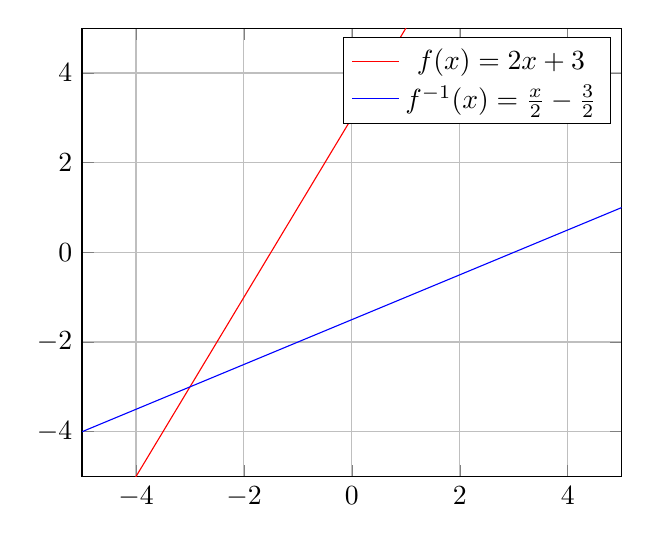
\begin{tikzpicture}
            \begin{axis}[
                grid=major,
                ymin=-5,
                ymax=5,
                xmin=-5,
                xmax=5,
            ]
                \addplot[
                    color = red,
                    samples = 100
                ]{2 * x + 3};
                \addlegendentry{\(f(x) = 2x + 3\)}
                \addplot[
                    color = blue,
                    samples = 100
                ]{x / 2 - 3 / 2};
                \addlegendentry{\(f^{-1}(x) = \frac{x}{2} - \frac{3}{2}\)}
            \end{axis}
        \end{tikzpicture}
        \caption{Grafovi funkcije i njenzinog inverzna} 
        \label{fig:template}
    \end{figure}